\documentclass[11pt, twocolumn, a4paper]{article}

\usepackage{graphicx}
\usepackage{booktabs}
\usepackage{multirow}
\usepackage{atlasphysics}
\setlength{\oddsidemargin}{0.0 cm}
\setlength{\evensidemargin}{0.0 cm}
\setlength{\topmargin}{-1cm}
\setlength{\textheight}{24 cm}
\setlength{\textwidth}{16 cm}

%\newcommand{\ttbarm}{\mathrm{t \overline{t} \; }}
%\newcommand{\ttbar}{$\mathrm{t \overline{t} \; }$}
%\newcommand{\ttbars}{${t \overline{t} \; }$}
%\newcommand{\ttW}{{t \overline{t} W }}
%\newcommand{\ttZ}{{t \overline{t} Z }}
\newcommand{\sevenTeV}{\ensuremath{7\tev}}
\newcommand{\eightTeV}{\ensuremath{8\tev}}
\newcommand{\sqrtsevenTeV}{\ensuremath{\sqrt{s} = 7\tev}}
\newcommand{\sqrteightTeV}{\ensuremath{\sqrt{s} = 8\tev}}
\renewcommand{\mH}{\ensuremath{m_{\Hboson}}}
\newcommand{\hgg}{\ensuremath{\Hboson \rightarrow \gamma\gamma \;}}
\newcommand{\hbb}{\ensuremath{\Hboson \rightarrow b\bar{b}}}
\newcommand{\htautau}{\ensuremath{\Hboson \rightarrow \tau\tau}}

\newcommand{\hWW}{\ensuremath{\Hboson \rightarrow WW}}
\newcommand{\ttH}{\ensuremath{\ttbar\Hboson}}
\newcommand{\bbH}{\ensuremath{b\bar{b}\Hboson}}
\newcommand{\tH}{\ensuremath{t\Hboson}}
\newcommand{\tHqb}{\ensuremath{t\Hboson{q}{b}}}
\newcommand{\WtH}{\ensuremath{Wt\Hboson}}
\newcommand{\BSMtH}{\ensuremath{{\rm BSM} \; \tH}}
\newcommand{\tbarH}{\ensuremath{\bar{t}\Hboson}}
\newcommand{\ggH}{ggF}
\newcommand{\VBFH}{VBF}
\newcommand{\WH}{\ensuremath{W\Hboson}}
\newcommand{\ZH}{\ensuremath{Z\Hboson}}
\newcommand{\qmutilde}{\ensuremath{\tilde{q}_{\mu}}}
\newcommand{\anti}{\scriptstyle\sim}
\newcommand{\meg}{\ensuremath{m_{e\gamma}}}
\newcommand{\mgamgam}{\ensuremath{m_{\gamma\gamma}}} 
\newcommand{\mgg}{\mgamgam}
\newcommand{\diphoton}{\ensuremath{\gamma\gamma\,}}
\newcommand{\muttH}{\ensuremath{\mu_{\ttH}}}
\newcommand{\muH}{\ensuremath{\mu}}


\pagestyle{plain}

\setlength{\parindent}{0in}

\usepackage[
  locale=DE,
  separate-uncertainty=true,
  decimalsymbol=.,
  per-mode=symbol-or-fraction,
]{siunitx}
\DeclareSIUnit\permille{\text{\textperthousand}}
\usepackage{textcomp}
\usepackage{amsmath,amssymb}

\usepackage[verbose]{placeins}

\begin{document}
\thispagestyle{empty}

\author{Salvatore La Cagnina}
\title{Summary of `Measurement of R = ${\mathcal{B}\left( t \rightarrow Wb \right)/\mathcal{B}\left(t \rightarrow Wq \right)} $ in Top--quark--pair Decays using Lepton+jets Events and the Full CDF Run II Data set'}
\maketitle
\vspace{-1cm}

This paper presents a simultaneous measurement of $R$ and the \ttbar production cross section $\sigma_{\ttbar}$.
R describes the fraction of the branching ratio with
\begin{equation*}
	R = \frac{\mathcal{B}\left(t \rightarrow Wb \right)}{\mathcal{B}\left(t \rightarrow Wq \right)} = \frac{\left|V_{tb}\right|^2}{\left|V_{tb}\right|^2+\left|V_{ts}\right|^2+\left|V_{td}\right|^2}
\end{equation*}
and is therefore also related to the elements of the Cabibbo-Kobayashi-Maskawa (CKM) matrix for the bottom like quarks with the top quark $(|W_{tq}|, q=d,s,b)$.
By using constrains on the CKM elements, $V_{ts}$ and $V_{td}$ the value for the $|V_{tb}|$ matrix element is close to one.
Consequently, any deviation of $R$ close to one would indicate an influence of new beyond Standard Model physics like additional quarks or non SM top quark production.
Since the $\sigma_{\ttbar}$ in other measurements is often calculated with $R=1$, $\sigma_{\ttbar}$ and $R$ are measured simultaneously, in order to avoid any bias.\\
The dataset is provided by the CDF II detector at the Fermilab Tevatron Collider and corresponds to an integrated luminosity of $\SI{8.7}{fb^{-1}}$.
The events are produced with $p\overline{p}$ collisions at a center of mass energy of $\sqrt{s} = \SI{1.96}{TeV}$.\\
In order to reproduce the $\ttbar\;$ signature the lepton + multiple jets decay channel is considered.
One of the $W$ bosons decays hadronically and one leponically into either a electron or muon.
Therefore, the topology of the analyzed channel consists of one lepton (electron or muon), one neutrino inducing missing transverse energy $E_T^\text{miss}$ and four jets of which two originate from the hadronization of $b$ quarks.\\
According to this topology the event selection is chosen to require one isolated lepton ($e$ or $\mu$) with transverse energy $E_T > \SI{20}{GeV}$, $E_T^\text{miss} > \SI{20}{GeV}$ and at least three jets.
The jets are required to have an $E_T$ greater then $\SI{30}{GeV}$, $\SI{25}{GeV}$ and $\SI{20}{GeV}$ for either the leading, sub-leading or any additional jet respectively.
Furthermore, one or two identified $b$ jets are required to be found.
In order to have a better reconstruction of the event, a selection criteria for the $W$ boson transverse mass greater then $\SI{20}{GeV}$ is added.\\
The remaining background contributions after the event selection are $W$ boson + heavy-flavor jets ($c$,$b$), $W$ + light-flavor jets, QCD multijet + leptons, diboson production, single-top-quark production and $Z$ boson + jets.
These backgrounds are estimated using either data based techniques, simulation based techniques or both (REF 10).\\
For the main analysis a simultaneous fit in 18 subsamples is performed.
These subsamples are created by separating the sample into their lepton category (electron, central or forward muon), the number of jets (3,4,$\geq$5) and the number of b tagged jets (2 b-tag, 3 b-tag).
It is noticeable that the number of b-tag jets is the most sensitive to changes in $R$, due to its influence in the number of decaying top quarks into b quarks.
Assuming a maximum efficiency for the b-tagging algorithm, the expected number of events with two b-tags would be proportional to $R^2$ , whereas, the number of events with one b-tag is proportional to $2R(1-R)$.
The total expected number of events $\mu_\text{exp}^{i,j}$ is determined using the expression
\begin{equation*}
	\mu_\text{exp}^{i,j} = \mu_{\ttbar}^{i,j} + N_B^{i,j} = \mathcal{L}^j \epsilon_\text{evt}^{i,j} \sigma_{\ttbar} \epsilon_\text{tag}^i(R) + N_B^{i,j},
\end{equation*}
where $i$ indicating the jet bin with either one or two b-tagged jets and $j$ indicating the lepton category.
$N_B^{i,j}$ is the expected number of background events, $\mathcal{L}^i$ the integrated luminosity, $\epsilon_\text{evt}^{i,j}$ the trigger and lepton identification efficiencies and $\epsilon_\text{tag}^i(R)$ is the event tagging efficiency.
In order to account for the monte carlo sample assuming $|V_{tb}|=1$ in the event generation, the matched parton level quarks are reassigned in their flavor if a random generated number $P_b$ is lower then the value chosen for $R$.
This creates a sample with an $R$ fraction of top quarks decaying into bottom quarks and a $(R-1)$ fraction decaying differently.\\
Having extracted the expected yields for the number of events a likelihood fit can be performed.
The used likelihood function is 
\begin{equation*}
	\mathcal{L}=\prod_{i,j}\mathcal{P}\left(\mu^{i,j}_{exp}(R,\sigma_{\ttbar},x_{a})|N^{i,j}_{obs}\right)\prod_{a}G\left(x_{a}|0,1\right),
\end{equation*}
which includes a Poission probability $\mathcal{P}\left(\mu^{i,j}_{exp}(R,\sigma_{\ttbar},x_{a})|N^{i,j}_{obs}\right)$ to observe $N^{i,j}_{obs}$ events with an expected number of $\mu^{i,j}_{exp}$.
The Gaussian functions $G\left(x_{a}|0,1\right)$ run over the nuisance parameters $x_a$ allowing to include sources of systematic uncertainties.
Since not all systematic uncertainties can be implemented as nuisance parameters, the analysis is executed by varying some uncertainties to determine their influence on the uncertainties on $R$ and $\sigma_{\ttbar}$.\\
The resulting values of the simultaneous fit in all the subsamples are $R = \num{0.94}\, \pm \,\num{0.09}$ and $\sigma_{\ttbar}=\SI{7.5 \pm 1.5}{pb}$ with a correlation of $\rho=-0.434$.
This result can be seen in fig. \ref{res} which 

\begin{figure}
	\centering
	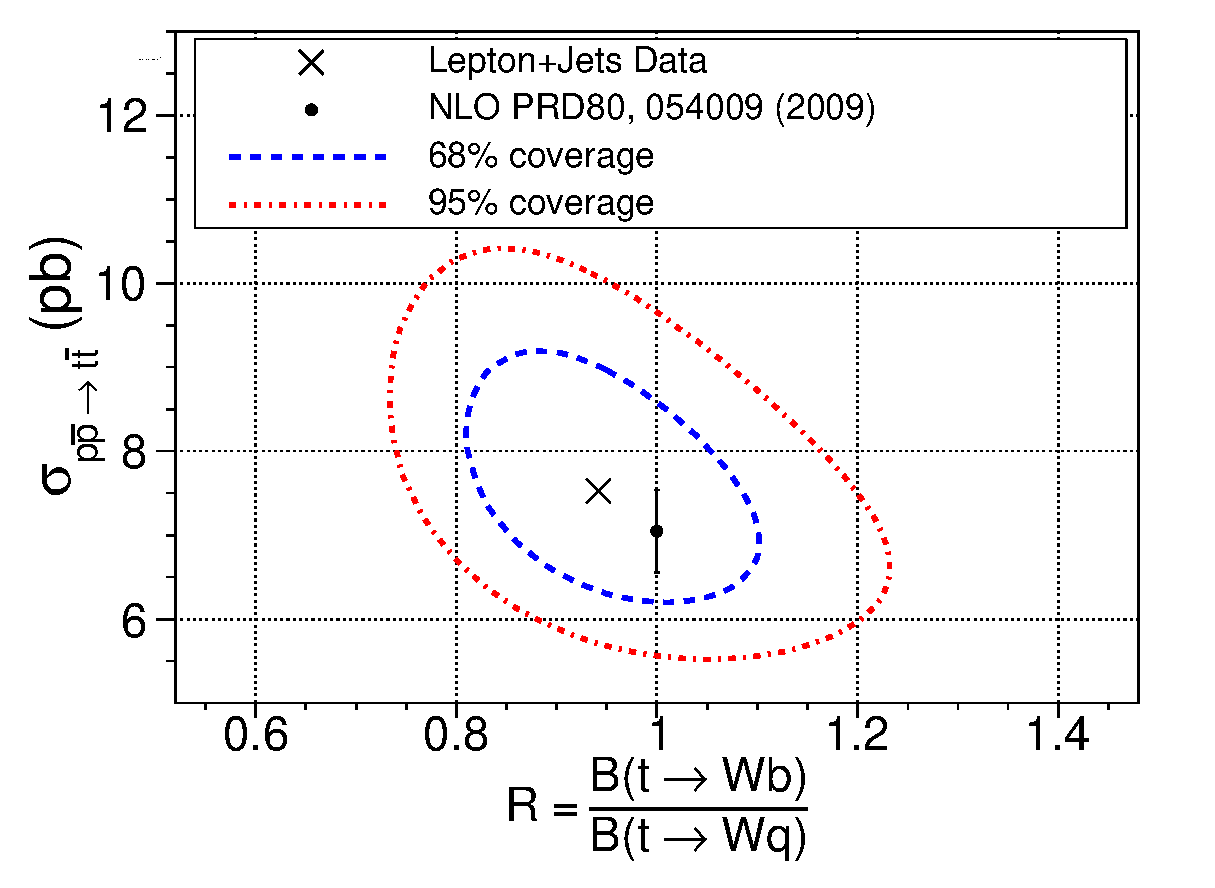
\includegraphics[width=0.5\textwidth]{contorni_corrected2.eps}
	\caption{The fit results for $R$ and $\sigma_{\ttbar}$ with its \SI{68}{\%} and \SI{95}{\%} confidence regions. The point corresponds to the theory NLO calculations.}
	\label{res}
\end{figure}

\begin{thebibliography}{99}
\bibitem{paper} ATLAS Collaboration,
\small{ Measurement of R = ${\mathcal{B}\left( t \rightarrow Wb \right)/\mathcal{B}\left(t \rightarrow Wq \right)} $ in Top--quark--pair Decays using Lepton+jets Events and the Full CDF Run II Data set}, Phys. Rev. D 87 (2013) 111101.
\end{thebibliography}



\end{document}


%\begin{figure}[ht!]
%  \begin{center}
%    \includegraphics[width=0.5\textwidth]{plot.pdf}
%    \caption{A figure caption~\cite{brandt}.}
%    \label{fig:fig1}
%  \end{center}
%\end{figure}














% In this paper a measurement of the $t \overline{t} Z$ and $t \overline{t} W$ production cross section is presented.
% The sample contains $\SI{3.2}{fb^{-1}}$ of $pp$ collision data at $\sqrt{s} = \SI{13}{TeV}$.
% The data is collected with the ATLAS detector at the LHC at CERN in the year 2015. 
% In order to extract the cross sections, a maximum-likelihood fit is used at differently selected signal and control regions.\\
% %
% %
% This measurement yields a test of the Standard Model (SM) due to new physics possibly changing the production of massive vector bosons together with \ttbars.
% Furthermore, this measurement offers information about the neutral-current coupling of the top quark which can be compared to theoretical SM predictions.
% This measurement has been previously studied for $7$ and $\SI{8}{TeV}$ \cite{paper_alt1,paper_alt2}, however, this study is performed with a higher center of mass energy leading to the increased cross sections of processes.\\
% %
% %
% For this measurement different decay channels are considered.
% They can be separated in three different categories.
% Those are same-sign muon (SS-$\mu$), trilepton and tetralepton.
% The decay requirements for the channels and their correspondence to $\ttW$ and $\ttZ$ can be seen in Table \ref{tab:intro-channels}.
% \begin{table}[htbp]
% \centering
% \caption{\label{tab:intro-channels} Decay modes with assignment to the $\ttW$ or $\ttZ$ process and corresponding channel.\cite{paper}} 
% \resizebox{0.5\textwidth}{!}{
% \begin{tabular}{cccc}
% \toprule
% Process & \ttbar decay & Boson decay & Channel\\
% \midrule
% \multirow{2}{*}{$\ttW$} 
% &  $(\mu^{\pm}\nu b) (q\bar{q} b) $ & $\mu^{\pm}\nu$ & SS dimuon\\
% & $ (\ell^{\pm}\nu b) (\ell^{\mp}\nu b)$ & $\ell^{\pm}\nu$ & Trilepton\\
% \midrule
% \multirow{2}{*}{$\ttZ$} 
% & $(\ell^{\pm}\nu b) (q\bar{q} b)$ & $ \ell^{+}\ell^{-}$ & Trilepton\\
% & $(\ell^{\pm}\nu b) (\ell^{\mp} \nu b)$ & $ \ell^{+}\ell^{-}$ & Tetralepton\\
% \bottomrule
% \end{tabular}}
% \end{table}
% Each of the analysis channels is divided in multiple signal, control and validation regions.
% For the cross sections the signal and control regions are fitted simultaneously.\\
% %
% %
% The monte carlo samples are created using several generators with fixed top and Higgs masses to $m_t=\SI{172.5}{GeV}$ and $m_H=\SI{125}{GeV}.$
% In order to correctly simulate the events, the main backgrounds have to be implemented.
% These are fake leptons, diboson events ($WZ,ZZ$) and other SM processes creating at least three prompt leptons like $Z$+jets or \ttbars + Higgs processes.\\
% \FloatBarrier
% %
% Requiring leptons to be prompt and therefore being isolated reduces the amount of lepton background from hadron decays and misidentified leptons.
% Other cuts and trigger requirement are also added in order to minimize the amount of background events.
% For the different analysis channels and the different signal and control regions different cuts are applied.\\
% The SS-$\mu$ channel has the highest sensitivity in comparison to other lepton channels due to the electron having a much higher charge misidentification.
% The events are chosen by using cuts on the transverse momentum $p_T$, missing transverse momentum $E_T^{miss}$, the scalar sum of $p_T$ called $H_T$ and the number of $b$-tagged jets. 
% The main background are fake leptons so the validation region is chosen so the background estimate which is extracted using the matrix method \cite{MM} can be approved.\\
% %
% In the trilepton channel there are four signal regions, one control region and two validation regions.
% The signal regions are distinguished by their number of $b$-tagged and light jets, by the presence of a $Z$ candidate and the sign of two same flavor leptons.
% This channel is sensitive to $\ttW$ and $\ttZ$ and its main background source is fake leptons but also other previously mentioned background.
% The requirements of this channel which suppresses most other background are one pair of opposite signed same flavor leptons (OSSF) and the invariant mass of them being near the $Z$ mass.
% This is valid for three of the four signal regions the last one having these requirements vetoed.
% The validation regions are used to confirm the background hypothesis and the control region is used to constrain the $WZ$ background normalization for the fit.\\
% %
% The tetralepton channel is used for $\ttZ$ and requires two pairs of (OSSF) leptons.
% Signal regions are chosen by the flavor of the pairs being identical or not and by the number of $b$-tagged jets leading to four different regions.
% The main background is again caused by fake leptons and is suppressed by applying cuts on $p_T$, $H_T$ and the invariant mass of the opposite signed lepton pairs.
% The control region is used to constrain the $ZZ$ background normalization for the fit analogously to the trilepton channel.\\
% %
% %
% The main systematic uncertainties are caused by the reconstruction of the physics object and fake leptons (for $\ttW$), however, the main uncertainty for this measurement is the static uncertainties caused by the overall acceptance of the processes of $\SI{6}{\permille}$ and $\SI{2}{\permille}$ for $\ttZ$ and $\ttW$ respectively.\\
% %
% %
% By simultaneously fitting the control and signal regions using a binned maximum-likelihood fit with systematic uncertainties as nuisance parameters, the cross sections can be extracted.
% They are measured to be 
% ${\sigma_{\ttZ}=\SI[parse-numbers=false]{0.92 \pm 0.29 (stat.) \pm 0.10 (syst.)}{pb}}$ and 
% ${\sigma_{\ttW}=\SI[parse-numbers=false]{1.50 \pm 0.72 (stat.) \pm 0.33 (syst.)}{pb}}$.
% These are consistent with the SM predictions which are calculated in NLO perturbative QCD to be
% ${\sigma_{\ttZ}=\SI[parse-numbers=false]{0.84 \pm 0.09}{pb}}$ and
% ${\sigma_{\ttW}=\SI[parse-numbers=false]{0.60 \pm 0.08}{pb}}$.
% This can also be seen in fig. \ref{fig:theo} since the SM prediction is contained in the $\SI{68}{\%}$ confidence level interval.
% Relying on this measurement, the significance over the background only hypothesis for $\ttW$ is only $\num{2.2}\sigma$ which is not high enough to approve the existence of the $\ttW$ process.
% This is mainly caused because of the high statistical uncertainty, therefore, further analysis with more data have to follow.
% \begin{figure}[h!]
% 	\centering
% 	\includegraphics[width=0.5\textwidth]{paper/ttZ_vs_ttW_2Dfit.pdf}
% 	\caption{Resulting cross section for $\ttW$ and $\ttZ$ compared to the SM prediction. The $\SI{68}{\%}$ and $\SI{95}{\%}$ confidence level for the fit and the one sigma uncertainty for the theory is shown. \cite{paper}}
% 	\label{fig:theo}
% \end{figure}
